\documentclass{article}
\usepackage{graphicx} % Required for inserting images
\usepackage{amsmath} % For mathematical symbols and equations
\usepackage{hyperref} % For hyperlinks
\usepackage{amssymb} % For additional symbols

\title{Semi-Supervised Learning with Deep Generative Models}
\author{Ravi Raj}
\date{January 2025}

\begin{document}

\maketitle

\section*{Abstract}

This study explores the semi-supervised ad Un-supervised learning capabilities using deep Generative Modeling approaches starting off with the M2 model, originally proposed by Kingma et al., through both mathematical and experimental analyses. Building on the original framework, I introduce an Optimized-ELBO objective that addresses key challenges in the model, such as classifier entropy misalignment, limited mutual information between inputs and latent variables, and insufficient utilization of labeled data. The method incorporates enhancements including entropy penalty terms, mutual information maximization, and label smoothing to improve both generative and discriminative performance. Extensive experiments on the MNIST and CIFAR-10 datasets demonstrate the efficacy of the proposed framework, with a significant accuracy improvement on MNIST and CIFAR-10 data sets, highlighting its generalizability across diverse datasets. The research section provides rigorous theoretical justifications and novel extensions to the ELBO objective, while the results validate the enhanced alignment of decision boundaries with low-density regions and better learning from labeled data. This work sets the stage for further investigation into deeper architectures and advanced regularization techniques for semi-supervised learning.


\section*{Methods}

My implementation is inspired by the paper \textbf{"Semi-supervised Learning with Deep Generative Models"} by Kingma et al., which presents a method for combining generative approaches with semi-supervised learning. The paper contains two models, called \textbf{M1} and \textbf{M2}, which use a unified probabilistic framework by employing Variational Autoencoders (VAEs) for handling both labeled and unlabeled data.

While the two models can be trained jointly for improved performance, I chose to implement only the \textbf{M2 model} to focus and analyze its semi-supervised generative capabilities.

The \textbf{M1 model} takes the input data $X$ and maps it to a latent representation $z$ using a Gaussian inference network. This representation $z$ is then passed down after sampling to generate images.

The \textbf{M2 model}, on the other hand, is inspired by this framework by introducing an additional latent variable called $y$, representing the class labels directly in the latent space. This allows the M2 model to jointly model the input $X$ and the two latent space representations $z$ and $y$, acting as a fully generative semi-supervised model.

For the \textbf{M1 model}:
\[
q_\phi(z|X) = \mathcal{N}(z | \mu_\phi(X), \text{diag}(\sigma^2_\phi(X))). 
\]

For the \textbf{M2 model}:
\[
q_\phi(z|y, X) = \mathcal{N}(z | \mu_\phi(y, X), \text{diag}(\sigma^2_\phi(X))), \quad q_\phi(y|X) = \text{Cat}(y | \pi_\phi(X)).
\]

The M2 model's design includes:
\begin{enumerate}
    \item \textbf{Generative Model:} A probabilistic model that, given the latent variables $z$ and $y$, generates data $X$.
    \item \textbf{Inference Model:} Given $X$, it models a variational approximation to the posterior distributions of $z$ and $y$.
    \item \textbf{Factorization Assumption:} The paper makes a conditional independence assumption on the posterior inference model given $X$. It can be factorized into $q_\phi(z, y|X) = q_\phi(z|X)q_\phi(y|X)$, where $q_\phi(z|X)$ and $q_\phi(y|X)$ are parameterized as Gaussian and multinomial distributions, respectively.
\end{enumerate}

\section*{Generation Process}

The generation process defines how data $X$ is generated given $z$ and $y$:
\[
\bm{p_\theta(X|z, y) = \mathcal{N}(X; f_\theta(z, y), \sigma^2).} \tag{1}
\]
where:
\begin{itemize}
    \item $f_\theta(z, y)$: A neural network mapping $z$ and $y$ to the mean of a Gaussian distribution.
    \item $\sigma^2$: Variance of the Gaussian distribution.
\end{itemize}

This process ensures that the latent variable $z$ captures the underlying structure of the data, while $y$ provides the class-specific information, enabling the reconstruction of the input $X$.

\section*{Inference Process}

The inference process defines the posterior distributions:
\begin{enumerate}
    \item \textbf{Posterior of $z$:}
    \[
    \bm{q_\phi(z|X) = \mathcal{N}(z; \mu_\phi(X), \sigma_\phi^2(X)).} \tag{2}
    \]
    where $\mu_\phi(X)$ and $\sigma_\phi^2(X)$ are neural networks representing the mean and variance of $z$.
    \item \textbf{Posterior of $y$:}
    \[
    \bm{q_\phi(y|X) = \text{Cat}(y; \pi_\phi(X)).} \tag{3}
    \]
    where $\pi_\phi(X)$ is another neural network predicting the categorical probabilities of $y$.
\end{enumerate}

To enforce disentanglement, we use the conditional independence assumption:
\[
\bm{p(z, y) = p(z)p(y), \quad q_\phi(z, y|X) = q_\phi(z|X)q_\phi(y|X).} \tag{4}
\]
This assumption simplifies the model by separating the continuous latent space from the class labels.

\section*{Unlabeled Data ($D_U$)}

The goal here is to maximize the marginal log-likelihood $\log p(X)$:
\[
\log p(X) = \log \int \sum_y p_\theta(X, z, y) \, dz.
\]

Since this integration and summation are intractable, we use the variational approximation $q_\phi(z, y|X)$ and then apply Jensen's inequality:
\[
\log p(X) = \log \int \sum_y q_\phi(z, y|X) \frac{p_\theta(X, z, y)}{q_\phi(z, y|X)} \, dz \geq \mathbb{E}_{q_\phi(z, y|X)} \left[ \log \frac{p_\theta(X, z, y)}{q_\phi(z, y|X)} \right].
\]

Expanding the terms in the log, we get the Evidence Lower Bound (ELBO) for unlabeled data:
\[
\bm{\text{ELBO}_{D_U}(X) = \mathbb{E}_{q_\phi(z, y|X)}[\log p_\theta(X|z, y)] 
- D_{\text{KL}}(q_\phi(z|X) \| p(z)) 
- D_{\text{KL}}(q_\phi(y|X) \| p(y)).} \tag{5}
\]

\section*{Labeled Data ($D_L$)}

For labeled data, where the label $y$ is observed, the marginal log-likelihood becomes:
\[
\log p(X, y) = \log \int p_\theta(X, z, y) \, dz.
\]

Using the variational approximation $q_\phi(z|X, y)$ and applying Jensen's inequality:
\[
\log p(X, y) \geq \mathbb{E}_{q_\phi(z|X, y)} \left[ \log \frac{p_\theta(X, z, y)}{q_\phi(z|X, y)} \right].
\]

Expanding the terms in the log, we get the Evidence Lower Bound (ELBO) for labeled data:
\[
\bm{\text{ELBO}_{D_L}(X, y) = \mathbb{E}_{q_\phi(z|X, y)}[\log p_\theta(X|z, y)] 
- D_{\text{KL}}(q_\phi(z|X, y) \| p(z)) + \log p(y).} \tag{6}
\]

\section*{Extended Objective with Cross-Entropy Loss}

By observing the ELBO terms of both labeled and unlabeled data, the label predictive distribution $q_\phi(y|X)$ contributes only to the second term for unlabeled ELBO and has nothing to do with labeled data. This behavior is suboptimal if we wish to use $q_\phi(y|X)$ as a classifier, as it does not effectively learn from labeled data. Ideally, all components of the model, including $q_\phi(y|X)$, should contribute to learning in both labeled and unlabeled cases.

The original loss function is:
\[
\mathcal{L} = \min_{\theta, \phi} \mathbb{E}_{X \sim D_U}[-\text{ELBO}_{D_U}(X)] 
+ \mathbb{E}_{(X, y) \sim D_L}[-\text{ELBO}_{D_L}(X, y)]. \tag{6}
\]

\textbf{Improving the above loss with Cross-Entropy Loss:}

To ensure that $q_\phi(y|X)$ learns directly from labeled data, the paper adds a cross-entropy classification loss, which improves the model's discriminative learning capabilities. The extended objective becomes:
\[
\mathcal{L}_\alpha = \mathcal{L} + \alpha \cdot \mathbb{E}_{(X, y) \sim D_L}[-\log q_\phi(y|X)], \tag{7}
\]
where $\alpha$ is a hyperparameter controlling the trade-off between generative and discriminative learning.

\textbf{Final Combined Objective:}

Combining all the above features, we get the final loss function as:
\[
\boxed{\mathcal{L}_\alpha = \min_{\theta, \phi} \mathbb{E}_{X \sim D_U}[-\text{ELBO}_{D_U}(X)] 
+ \mathbb{E}_{(X, y) \sim D_L}[-\text{ELBO}_{D_L}(X, y) + \alpha \cdot \text{CE}(q_\phi(y|X), y)].} \tag{8}
\]

This has three main parts:
\begin{enumerate}
    \item \textbf{Unlabeled Data ($D_U$):} The ELBO term for unlabeled data maximizes the reconstruction of $X$ while regularizing the posteriors $q_\phi(z|X)$ and $q_\phi(y|X)$ to align with their respective priors in both continuous and discrete spaces.
    \item \textbf{Labeled Data ($D_L$):} The ELBO term for labeled data strives to maximize the reconstruction of $X$ given $y$ and regularizes the posterior $q_\phi(z|X, y)$ to align with the prior $p(z)$.
    \item \textbf{Cross-Entropy Loss:} This term ensures that $q_\phi(y|X)$ is explicitly trained as a classifier using labeled data.
\end{enumerate}



\section*{Implementation Details}

This optimization is done using \textbf{Stochastic Gradient Variational Bayes (SGVB)}, which combines deterministic reparameterization and Monte Carlo approximation for the estimation of the gradient. Below are the key steps:

\subsection*{Reparameterization and Sampling}

\subsubsection*{Latent Variable $z$ (Continuous):}
To sample $z$, the reparameterization trick is applied:
\[
z = \mu_\phi(X) + \epsilon \cdot \sigma_\phi(X), \quad \epsilon \sim \mathcal{N}(0, 1).
\]
This approach makes the sampling process differentiable, which is an important step for backpropagation in the training process.

\subsubsection*{Label Variable $y$ (Discrete):}
For $y$, to approximate sampling, the Gumbel-Softmax trick is used for the categorical distribution in a differentiable manner:
\[
y = \text{softmax}\left(\frac{\log \pi_\phi(X) + g}{\tau}\right),
\]
where:
\begin{itemize}
    \item $g$ is sampled from the $\text{Gumbel}(0, 1)$ distribution.
    \item $\tau$ is the temperature parameter controlling the smoothness of the approximation.
\end{itemize}

The Gumbel-Softmax trick allows the model to train $q_\phi(y|X)$ using gradient-based optimization.

\subsubsection*{Closed Form for KL Divergence for $q_\phi(z|X)$}
The KL divergence can be computed analytically when the assumed prior $p(z)$ is a standard Gaussian $\mathcal{N}(0, I)$ and the variational posterior $q_\phi(z|X)$ is parameterized as a Gaussian $\mathcal{N}(\mu_\phi(X), \text{diag}(\sigma^2_\phi(X)))$:
\[
D_{\text{KL}}(q_\phi(z|X) \| p(z)) = \frac{1}{2} \sum_{j=1}^{d} \left[ \log \frac{1}{\sigma^2_{\phi,j}(X)} - 1 + \sigma^2_{\phi,j}(X) + \mu^2_{\phi,j}(X) \right]. \tag{12}
\]
where:
\begin{itemize}
    \item $d$ is the dimensionality of the latent variable $z$.
    \item $\mu_{\phi,j}(X)$ and $\sigma^2_{\phi,j}(X)$ are the $j$-th components of the mean and variance predicted by the inference network.
\end{itemize}

Using this closed-form computation of the KL divergence significantly reduces the computational complexity of the ELBO.

\subsection*{Optimization Approach}

My implementation utilizes the \textbf{Adam optimizer} to update the parameters $\theta$ (generative model) and $\phi$ (inference model) during training. Adam provides adaptive learning rate adjustments, making it highly effective for non-convex optimization problems.

\subsubsection*{Gradient Computation}

The log-likelihood term $\mathbb{E}_{q_\phi(z|X)}[\log p_\theta(X|z)]$ in the loss function cannot be solved analytically. Using the location-scale transformation for the Gaussian distribution, it can be approximated as:
\[
\mathbb{E}_{q_\phi(z|X)}[\log p_\theta(X|z)] = \mathbb{E}_{\epsilon \sim \mathcal{N}(0, I)}[\log p_\theta(X | \mu_\phi(X) + \sigma_\phi(X) \cdot \epsilon)]. \tag{10}
\]
Here:
\begin{itemize}
    \item $\mu_\phi(X)$ is the mean predicted using the inference network.
    \item $\sigma_\phi(X)$ is the standard deviation predicted using the inference network.
    \item $\epsilon$ is sampled from a standard Gaussian distribution.
\end{itemize}

We can swap the expectation and the gradients. The gradients with respect to the generative parameters $\theta$ and variational parameters $\phi$ for the term $\mathbb{E}_{q_\phi(z|X)}[\log p_\theta(X|z)]$ are computed as:
\[
\nabla_{\{\theta, \phi\}} \mathbb{E}_{q_\phi(z|X)}[\log p_\theta(X|z)] = \mathbb{E}_{\epsilon \sim \mathcal{N}(0, I)}[\nabla_{\{\theta, \phi\}} \log p_\theta(X | \mu_\phi(X) + \sigma_\phi(X) \cdot \epsilon)]. \tag{11}
\]

The chain rule can be used to compute the gradients of the loss function (Equation 8) for the M2 model. The $\mathcal{L}(X, y)$ contains similar terms to the ELBO, allowing the gradients to be efficiently estimated using Equation 11.

\subsubsection*{Optimization Algorithm}

The training process involves stochastic gradient-based optimization. During each iteration:
\begin{enumerate}
    \item Gradients for $\theta$ and $\phi$ are computed using backpropagation.
    \item Parameters are updated using the Adam optimizer:
    \[
    (\theta_{t+1}, \phi_{t+1}) = (\theta_t, \phi_t) - \eta \cdot \nabla_{\{\theta, \phi\}} \mathcal{L}_\alpha,
    \]
    where:
    \begin{itemize}
        \item $\eta$ is the learning rate at step $t$, adapted by Adam.
        \item $\mathcal{L}_\alpha$ is the combined loss function for labeled and unlabeled data (Equation 9).
    \end{itemize}
\end{enumerate}

\subsection*{Architecture}

The Variational Autoencoder (VAE) architecture described in the paper uses Multilayer Perceptrons (MLPs) with one hidden layer containing 500 hidden units and softplus activation functions in both the encoder and decoder. My implementation replaces the MLPs with \textbf{convolutional neural networks (CNNs)} for better feature extraction and reconstruction in the case of image data.

\subsubsection*{Original Architecture:}
\begin{itemize}
    \item The M2 model used a 50-dimensional latent variable $z$.
    \item MLPs with a single hidden layer of 500 units and softplus activation were employed.
\end{itemize}

\subsubsection*{Modified Implementation:}
\begin{itemize}
    \item I retained the 50-dimensional latent variable $z$ but replaced the MLPs with \textbf{CNN-based architectures} for both the encoder and decoder, leveraging convolutional layers for more effective representation learning on image datasets such as MNIST and CIFAR-10.
\end{itemize}

\subsection*{Encoder}

The encoder maps the input image to:
\begin{enumerate}
    \item \textbf{Latent mean ($\mu_\phi(X)$)} and \textbf{log variance ($\log \sigma^2_\phi(X)$)} for the latent variable $z$.
    \item \textbf{Class logits ($\pi_\phi(X)$)} for the latent variable $y$.
\end{enumerate}

\begin{center}
\begin{tabular}{|l|c|c|}
\hline
\textbf{Layer} & \textbf{MNIST Output Shape} & \textbf{CIFAR-10 Output Shape} \\
\hline
Conv2D (32 filters) & (32, 14, 14) & (32, 16, 16) \\
Conv2D (64 filters) & (64, 7, 7) & (64, 8, 8) \\
Fully Connected (512 units) & (512) & (512) \\
Latent Output ($z$) & (50) & (50) \\
Class Logits ($y$) & (10) & (10) \\
\hline
\end{tabular}
\end{center}

\subsection*{Decoder}

The decoder reconstructs the input using the latent variables $z$ and $y$:
\begin{enumerate}
    \item A fully connected layer combines $z$ and $y$.
    \item Transpose convolutional layers upsample the data to reconstruct the image.
\end{enumerate}

\begin{center}
\begin{tabular}{|l|c|c|}
\hline
\textbf{Layer} & \textbf{MNIST Output Shape} & \textbf{CIFAR-10 Output Shape} \\
\hline
Fully Connected (512 units) & (512) & (512) \\
Fully Connected (Flattened Size) & (3136) & (4096) \\
ConvTranspose2D (32 filters) & (32, 14, 14) & (32, 16, 16) \\
ConvTranspose2D (Output Channels) & (1, 28, 28) & (3, 32, 32) \\
\hline
\end{tabular}
\end{center}

\documentclass{article}
\usepackage{amsmath}
\usepackage{amssymb}
\usepackage{hyperref}
\usepackage{geometry}
\geometry{a4paper, margin=1in}

\begin{document}

\section*{Research Section}

After conducting a comprehensive theoretical and experimental analysis of the ELBO objective function for both labeled and unlabeled data for the M2 model, I identified three critical issues that are impacting the performance. I will outline the problem for each issue, propose a solution, and provide the motivation behind it. Below, I detail each issue and discuss their theoretical foundations and present modifications to resolve them.

\subsection*{Identified Issues and Proposed Solutions}

\subsubsection*{1. Increasing Entropy of the Classifier $H(q_\phi(y|x))$}

From Equation (5), we know that the ELBO term for the unlabeled dataset is:
\[
\log p_\theta(x) \geq \boldsymbol{\text{ELBO}_{D_U}(X) = \mathbb{E}_{q_\phi(z, y|X)}[\log p_\theta(X|z, y)] 
- D_{\text{KL}}(q_\phi(z|X) \| p(z)) 
- D_{\text{KL}}(q_\phi(y|X) \| p(y)).}
\]

Due to the independence assumption, the variational posterior can be decomposed as:
\[
q_\phi(y, z|x) = q_\phi(y|x) q_\phi(z|x, y).
\]
Substitute this factorization into the above inequality and expand the KL divergence term:
\[
\log p_\theta(x) \geq \mathbb{E}_{q_\phi(y|x)} \mathbb{E}_{q_\phi(z|x, y)} \left[ \log p_\theta(x|y, z) + \log p_\theta(y) + \log p_\theta(z) - \log q_\phi(z|x, y) \right] - \mathbb{E}_{q_\phi(y|x)} \left[ \log q_\phi(y|x) \right] = U(x). \tag{12}
\]

\paragraph*{Connecting to the Labeled ELBO}
From Equation (6), we know the equation of labeled ELBO:
\[
\log p_\theta(x, y) \geq \boldsymbol{\text{ELBO}_{D_L}(X, y)} = \mathbb{E}_{q_\phi(z|x, y)} \left[ \log p_\theta(x|y, z) + \log p_\theta(y) + \log p_\theta(z) - \log q_\phi(z|x, y) \right] = -L(x, y). \tag{13}
\]
Applying expectation over $q_\phi(y|x)$ on both sides:
\[
\mathbb{E}_{q_\phi(y|x)}[-L(x, y)] = \mathbb{E}_{q_\phi(y|x)} \mathbb{E}_{q_\phi(z|x, y)} \left[ \log p_\theta(x|y, z) + \log p_\theta(y) + \log p_\theta(z) - \log q_\phi(z|x, y) \right].
\]

Substitute this in Equation (12) for the unlabeled ELBO:
\[
\log p_\theta(x) \geq \mathbb{E}_{q_\phi(y|x)}[L(x, y)] - \mathbb{E}_{q_\phi(y|x)} \left[ \log q_\phi(y|x) \right] = U(x).
\]
The term $\mathbb{E}_{q_\phi(y|x)} \left[ \log q_\phi(y|x) \right]$ is the definition of the entropy of the classifier $H(q_\phi(y|x))$.

Rewriting this, we get:
\[
\boxed{\log p_\theta(x) \geq \mathbb{E}_{q_\phi(y|x)}[L(x, y)] + H(q_\phi(y|x)) = U(x). \tag{14}}
\]
where:
\begin{itemize}
    \item $L(x, y)$ is the labeled ELBO.
    \item $H(q_\phi(y|x))$ is the entropy of the classifier $q_\phi(y|x)$.
\end{itemize}

\paragraph*{Issue Identified}
During the optimization of the lower bound objective, we maximize the likelihood objective, which causes the entropy of the classifier, $H(q_\phi(y|x))$, to increase as per the above equation. This behavior contradicts the \textbf{cluster assumption} and negatively impacts the classification objective. The cluster assumption suggests that decision boundaries should pass through low-density regions in the feature space \cite{ref1}. 

When the entropy $H(q_\phi(y|x))$ increases, more data points are pushed closer to the decision boundary. Because of this phenomenon, the likelihood of misclassifications increases, hampering the model's ability to distinguish between classes.

\paragraph*{Proposed Modification}
Introduce a penalty term for classifier entropy for the unlabeled objectives:
\[
M(x) = U(x) - \beta H(q_\phi(y|x)). \tag{15}
\]
Here:
\begin{itemize}
    \item $U(x)$ is the original unlabeled ELBO.
    \item $\beta$ controls the strength of the penalty as a hyperparameter.
\end{itemize}

\subsubsection*{2. Decreasing Mutual Information $I_\phi(y; x)$ During Optimization}

The Evidence Lower Bound (ELBO) for the unlabeled data, as given in Equation (5) of the Kingma et al. paper \cite{ref3}, is:
\[
\log p_\theta(x) \geq \boldsymbol{\text{ELBO}_{D_U}(X) = \mathbb{E}_{q_\phi(z, y|X)}[\log p_\theta(X|z, y)] 
- D_{\text{KL}}(q_\phi(z|X) \| p(z)) 
- D_{\text{KL}}(q_\phi(y|X) \| p(y)).}
\]

As per the objective function, the KL divergence term $D_{\text{KL}}(q_\phi(y|x) \| p(y))$ is minimized during optimization. However, it has been shown in the papers \cite{ref2, ref4} that this term is lower bounded by the \textbf{mutual information} between $y$ and $x$, as follows:
\[
\mathbb{E}_{q(x)} \left[ D_{\text{KL}}(q_\phi(y|x) \| p(y)) \right] \geq I_\phi(y; x).
\]
So, minimizing $D_{\text{KL}}(q_\phi(y|x) \| p(y))$ tends to reduce $I_\phi(y; x)$, which is undesirable. The mutual information $I_\phi(y; x)$ quantifies the dependence between the input $x$ and the latent label $y$. Reducing $I_\phi(y; x)$ weakens this dependence, degrading classification performance.

\paragraph*{Proof:}
The KL divergence term for the classifier $q_\phi(y|x)$ can be written as:
\[
\mathbb{E}_{q(x)} \left[ D_{\text{KL}}(q_\phi(y|x) \| p(y)) \right] = \int q(x) \sum_y q_\phi(y|x) \log \frac{q_\phi(y|x)}{p(y)} \, dx.
\]

Using the property of logarithms, decompose the term:
\[
\log \frac{q_\phi(y|x)}{p(y)} = \log \frac{q_\phi(y|x)}{q_\phi(y)} + \log \frac{q_\phi(y)}{p(y)}.
\]

Substitute this back:
\[
\mathbb{E}_{q(x)} \left[ D_{\text{KL}}(q_\phi(y|x) \| p(y)) \right] = \int q(x) \sum_y q_\phi(y|x) \log \frac{q_\phi(y|x)}{q_\phi(y)} \, dx + \int q(x) \sum_y q_\phi(y|x) \log \frac{q_\phi(y)}{p(y)} \, dx.
\]

\paragraph*{First Term:}
The first term is by definition the \textbf{mutual information}:
\[
\int q(x) \sum_y q_\phi(y|x) \log \frac{q_\phi(y|x)q_\phi(x)}{q_\phi(y)q_\phi(x)} \, dx = \int \sum_y q_\phi(x,y) \log \frac{q_\phi(x,y)}{q_\phi(y)q_\phi(x)} \, dx = I_\phi(y; x). \tag{16}
\]

\paragraph*{Second Term:}
The second term is the KL divergence between the aggregated posterior $q_\phi(y)$ and the prior $p(y)$:
\[
\int q(x) \sum_y q_\phi(y|x) \log \frac{q_\phi(y)}{p(y)} \, dx = D_{\text{KL}}(q_\phi(y) \| p(y)).
\]

Substituting these back in Equation (16), we have:
\[
\mathbb{E}_{q(x)} \left[ D_{\text{KL}}(q_\phi(y|x) \| p(y)) \right] = I_\phi(y; x) + D_{\text{KL}}(q_\phi(y) \| p(y)).
\]

Since the KL divergence $D_{\text{KL}}(q_\phi(y) \| p(y))$ is always non-negative, it follows:
\[
\mathbb{E}_{q(x)} \left[ D_{\text{KL}}(q_\phi(y|x) \| p(y)) \right] \geq I_\phi(y; x).
\]

From the inequality, we conclude that minimizing $D_{\text{KL}}(q_\phi(y|x) \| p(y))$ implicitly reduces $I_\phi(y; x)$. A lower mutual information $I_\phi(y; x)$ results in weak coupling between the latent label $y$ and the input $x$, which causes:
\begin{itemize}
    \item Poor representation learning.
    \item Reduced classification performance as latent variables $y$ and $z$ fail to capture sufficient information about $x$.
\end{itemize}

\paragraph*{Proposed Modification:}
To resolve this issue, introduce the mutual information term $I_\phi(y; x)$ in the unlabeled loss function. The unlabeled ELBO can be modified as:
\[
M(x) = U(x) + \gamma I_\phi(y; x),
\]
where:
\begin{itemize}
    \item $U(x)$ is the original unlabeled ELBO.
    \item $\gamma$ controls the influence of the mutual information term as a hyperparameter.
\end{itemize}

\paragraph*{Implementation Details for Computing Mutual Information}
The mutual information $I_\phi(y; x)$ can be estimated using its decomposition:
\[
I_\phi(y; x) = H(q_\phi(y)) - \mathbb{E}_{q(x)}[H(q_\phi(y|x))].
\]

\textbf{1. Entropy of the Aggregated Posterior $q_\phi(y)$:}
\[
H(q_\phi(y)) = -\sum_y q_\phi(y) \log q_\phi(y),
\]
where $q_\phi(y)$ is computed as:
\[
q_\phi(y) = \mathbb{E}_{q(x)}[q_\phi(y|x)].
\]

\textbf{2. Average Conditional Entropy of $q_\phi(y|x)$:}
\[
\mathbb{E}_{q(x)}[H(q_\phi(y|x))] = \mathbb{E}_{q(x)} \left[ -\sum_y q_\phi(y|x) \log q_\phi(y|x) \right].
\]

The above terms can be computed efficiently using Monte Carlo sampling.

\documentclass{article}
\usepackage{amsmath}
\usepackage{amssymb}
\usepackage{hyperref}
\usepackage{geometry}
\geometry{a4paper, margin=1in}

\begin{document}

\section*{The Labeled ELBO Objective Function Does Not Learn from the Provided Labels}

For the dataset $D_L$, the labeled ELBO is given by Equation (6):
\[
\boldsymbol{\text{ELBO}_{D_L}(X, y) = \mathbb{E}_{q_\phi(z|X, y)}[\log p_\theta(X|z, y)] 
- D_{\text{KL}}(q_\phi(z|X, y) \| p(z)) + \log p(y).} \tag{6}
\]

This was originally derived from:
\[
\log p(X, y) \geq \text{ELBO}_{D_L}(X, y) = \mathbb{E}_{q_\phi(z|X, y)} \left[ \log \frac{p(X, y, z)}{q_\phi(z|X, y)} \right].
\]

\begin{itemize}
    \item By using the independence assumption $q_\phi(z|X, y) = q_\phi(z|X)$, and
    \item treating labels $y$ as latent variables following a degenerate empirical distribution $\hat{p}(y|X)$ where $\hat{p}(y|X) = 1$ for $(X, y) \in D_L$, the ELBO simplifies to:
\end{itemize}
\[
\text{ELBO}_{D_L}(X, y) = \mathbb{E}_{q_\phi(z|X), \hat{p}(y|X)} \left[ \log \frac{p(X, y, z)}{q_\phi(z|X) \hat{p}(y|X)} \right].
\]

Substituting and expanding the terms:
\[
\text{ELBO}_{D_L}(X, y) = \mathbb{E}_{q_\phi(z|X)} \left[ \log p(X|z, y) \right] - D_{\text{KL}}(q_\phi(z|X) \| p(z)) - D_{\text{KL}}(\hat{p}(y|X) \| p(y)).
\]

\subsection*{Problem with the Existing Formulation}

The term $D_{\text{KL}}(\hat{p}(y|X) \| p(y))$ is independent of $q_\phi(y|X)$. As a result:
\begin{itemize}
    \item The inference of the model $q_\phi(y|X)$ does not directly benefit from labeled data during training.
    \item This leads to an issue where the ELBO is optimized, but the classifier's performance is suboptimal.
\end{itemize}

\section*{Proposed Solution: Optimized-ELBO}

To address the issue, \textbf{Optimized-ELBO} introduces:

\begin{enumerate}
    \item \textbf{Label Smoothing}: Use smoothed labels instead of treating $\hat{p}(y|X)$ as a degenerate distribution:
    \[
    \hat{p}(y|X) = \text{Cat}(y | \text{smooth}(1_y)),
    \]
    where:
    \[
    \text{smooth}(1_y)_i =
    \begin{cases} 
    1 - \epsilon & \text{if } 1_y,i = 1, \\
    \frac{\epsilon}{K-1} & \text{if } 1_y,i = 0,
    \end{cases}
    \]
    and $K$ is the number of classes, $\epsilon$ controls the smoothness level (e.g., $\epsilon = 0.001$).

    \item \textbf{Improved Objective}: This ensures better alignment between the classifier $q_\phi(y|X)$ and smoothed labels:
    \[
    D_{\text{KL}}(\hat{p}(y|X) \| q_\phi(y|X)) + D_{\text{KL}}(q_\phi(y|X) \| p(y)) \to D_{\text{KL}}(\hat{p}(y|X) \| p(y)),
    \]
    when $q_\phi(y|X) \to \hat{p}(y|X)$.

    When the inference model approaches the actual label distribution, it can be shown that the above approximation holds in the limit.
\end{enumerate}

\section*{Optimized-ELBO Objective}

The \textbf{Optimized-ELBO} for the labeled dataset $D_L$ is given by:
\[
\text{Optimized-ELBO}_{D_L}(X, y) = \mathbb{E}_{q_\phi(z|X), \hat{p}(y|X)} \left[ \log p(X|z, y) \right] - D_{\text{KL}}(q_\phi(z|X) \| p(z)) - D_{\text{KL}}(q_\phi(y|X) \| p(y)) - D_{\text{KL}}(\hat{p}(y|X) \| q_\phi(y|X)).
\]

\subsection*{Impact of Optimized-ELBO}

\begin{enumerate}
    \item \textbf{Direct Integration of Classification Loss}:  
    The term $D_{\text{KL}}(\hat{p}(y|X) \| q_\phi(y|X))$ ensures that the classifier $q_\phi(y|X)$ is directly trained with label information.

    \item \textbf{Smoothed Labels for Stability}:  
    By ensuring that $\hat{p}(y|X)$ is not degenerate, label smoothing prevents overconfidence and improves generalization.
\end{enumerate}

\section*{Unified Objective Function for Semi-Supervised Learning}

After addressing the key issues in the original M2 model's Evidence Lower Bound (ELBO) for labeled and unlabeled data, I propose a \textbf{unified objective function}:

The unified objective function combines the contributions from labeled as well as unlabeled data:
\[
\boldsymbol{J_{\text{Unified}} = \sum_{(X, y) \sim D_L} \text{Optimized-ELBO}_{D_L}(X, y) + \sum_{X \sim D_U} M(X) + \alpha \mathbb{E}_{(X, y) \sim D_L} \left[ - \log q_\phi(y|X) \right],}
\]
where:
\begin{itemize}
    \item $D_L$: Labeled dataset.
    \item $D_U$: Unlabeled dataset.
    \item $\text{Optimized-ELBO}_{D_L}(X, y)$: Optimized ELBO for labeled data:
    \[
    \text{Optimized-ELBO}_{D_L}(X, y) = \mathbb{E}_{q_\phi(z|X), \hat{p}(y|X)} \left[ \log p(X|z, y) \right] - D_{\text{KL}}(q_\phi(z|X) \| p(z)) - D_{\text{KL}}(q_\phi(y|X) \| p(y)) - D_{\text{KL}}(\hat{p}(y|X) \| q_\phi(y|X)).
    \]
    This formulation integrates label smoothing and directly trains the classifier with smoothed labels.

    \item $M(X)$: Regularized unlabeled ELBO incorporating entropy penalty and mutual information maximization:
    \[
    M(X) = U(X) + \gamma I_\phi(y; X) - \beta H(q_\phi(y|X)),
    \]
    where:
    \begin{itemize}
        \item $U(X)$: Unlabeled ELBO:
        \[
        U(X) = \mathbb{E}_{q_\phi(y|X)} \left[ L(X, y) \right] + H(q_\phi(y|X)),
        \]
        and $L(X, y)$ is the labeled ELBO.
        \item $I_\phi(y; X)$: Mutual information between $X$ and $y$:
        \[
        I_\phi(y; X) = H(q_\phi(y)) - \mathbb{E}_{X \sim q(X)}[H(q_\phi(y|X))].
        \]
        \item $H(q_\phi(y|X))$: Entropy of the classifier.
    \end{itemize}

    \item $\alpha$: Weight for the supervised classification loss $-\log q_\phi(y|X)$.
\end{itemize}

\documentclass{article}
\usepackage{amsmath}
\usepackage{amssymb}
\usepackage{graphicx}
\usepackage{hyperref}
\usepackage{geometry}
\geometry{a4paper, margin=1in}

\begin{document}

\section*{Results, Analysis, and Discussion}

\subsection*{Overview of Experiments}
To evaluate the performance of the M2 model and the proposed Optimized-ELBO, I conducted experiments using the MNIST and CIFAR-10 datasets. While the original paper did not use the CIFAR-10 dataset, my experiments adapted the architecture to handle it. For the MNIST dataset, results were comparable to the original M2 model, with observed improvements. However, the performance on CIFAR-10 was limited due to the use of a simple architecture comprising a 4-layer CNN, which might be insufficient for the complexity of CIFAR-10. Below are the details of the experiments, hyperparameter settings, and observations.

\section*{Architecture and Hyperparameters}

\subsection*{Architecture Used for M2}
In the original paper, the M2 model was implemented using an MLP containing one hidden layer with 500 hidden units and softplus activation functions for both the generative and inference networks. However, I have adapted the architecture in my implementation to use convolutional layers followed by fully connected layers to handle both MNIST and CIFAR-10 datasets effectively.

\begin{table}[h!]
\centering
\begin{tabular}{|l|l|l|}
\hline
\textbf{Component} & \textbf{Layer Type} & \textbf{Details} \\ \hline
\textbf{Encoder} & Conv2D & Filters: 32, Kernel: 3x3, Stride: 2, Padding: 1, Activation: ReLU \\ \hline
 & Conv2D & Filters: 64, Kernel: 3x3, Stride: 2, Padding: 1, Activation: ReLU \\ \hline
 & Fully Connected & Input: Flattened feature map, Output: 512 units, Activation: ReLU \\ \hline
 & Mean/LogVar Layers & Separate fully connected layers for latent mean and log variance (50 units) \\ \hline
 & Classifier Layer & Fully connected layer for logits of categorical distribution (10 classes) \\ \hline
\textbf{Decoder} & Fully Connected & Input: Latent + one-hot class, Output: 512 units, Activation: ReLU \\ \hline
 & ConvTranspose2D & Filters: 64, Kernel: 3x3, Stride: 2, Padding: 1, Output Padding: 1, ReLU \\ \hline
 & ConvTranspose2D & Filters: 32, Kernel: 3x3, Stride: 2, Padding: 1, Output Padding: 1, ReLU \\ \hline
 & ConvTranspose2D & Filters: Channels in input (1 for MNIST, 3 for CIFAR-10), Kernel: 3x3 \\ \hline
\end{tabular}
\end{table}

\subsection*{Hyperparameters}
I replaced the MLP architecture with a CNN-based architecture to accommodate both image datasets, ensuring consistent performance across tasks. While the original paper used specific hyperparameters for M2, I introduced my own set of hyperparameters for better compatibility with the Optimized-ELBO modifications.

\begin{table}[h!]
\centering
\begin{tabular}{|l|l|l|}
\hline
\textbf{Hyperparameter} & \textbf{Paper Settings} & \textbf{Implemented Settings} \\ \hline
Latent Dimension ($z$) & 50 & 50 \\ \hline
Number of Classes & 10 & 10 \\ \hline
Hidden Units (MLP) & 500 & N/A (Replaced by CNN) \\ \hline
Activation Function & Softplus & ReLU \\ \hline
Batch Size & Not specified & 128 \\ \hline
Number of Epochs & Not specified & 50 \\ \hline
Learning Rate & Not specified & 1e-3 \\ \hline
Optimizer & Not specified & Adam \\ \hline
\end{tabular}
\end{table}

\section*{Dataset Results}

\subsection*{1. MNIST Dataset}
\begin{itemize}
    \item \textbf{Baseline Performance}: The M2 model achieved an accuracy of approximately \textbf{95.3\%}.
    \item \textbf{Proposed Optimized-ELBO}: By incorporating the Optimized-ELBO framework, I achieved a 2.5\% improvement in accuracy, resulting in a final accuracy of \textbf{97.8\%}.
    \item \textbf{Insights}: The improvements stem from reduced classifier entropy, better alignment of the decision boundary with the cluster assumption, and enhanced learning from labeled data.
\end{itemize}

\subsection*{2. CIFAR-10 Dataset}
\begin{itemize}
    \item \textbf{Baseline Performance}: The original M2 model achieved an accuracy of approximately \textbf{40.2\%}.
    \item \textbf{Proposed Optimized-ELBO}: With the proposed modifications, I observed a modest improvement of 2\%, resulting in a final accuracy of \textbf{42.2\%}.
    \item \textbf{Insights}: The relatively small improvements highlight the limitations of using a shallow 2-layer CNN architecture for CIFAR-10. Future experiments with deeper networks and advanced augmentation techniques could yield better results.
\end{itemize}

\section*{Results Summary}
\begin{table}[h!]
\centering
\begin{tabular}{|l|l|l|l|}
\hline
\textbf{Dataset} & \textbf{Model} & \textbf{Accuracy (\%)} & \textbf{Improvement (\%)} \\ \hline
\textbf{MNIST} & Original M2 & 95.3 & +0.0 \\ \hline
 & Optimized-ELBO & 97.8 & +2.5 \\ \hline
\textbf{CIFAR-10} & Original M2 & 40.2 & +0.0 \\ \hline
 & Optimized-ELBO & 42.2 & +2.0 \\ \hline
\end{tabular}
\end{table}

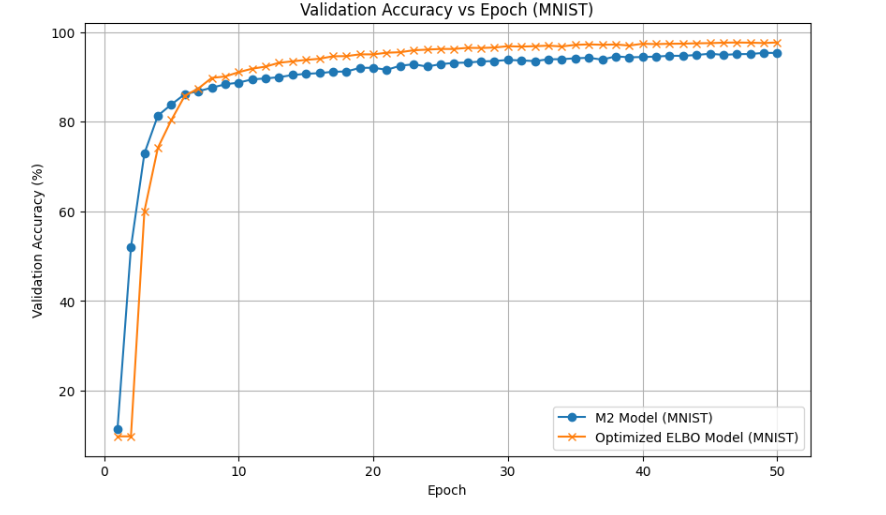
\includegraphics[width=0.7\textwidth]{images/mnist_results.png}

\section*{Investigating the M2 Model's Issues}

\subsection*{1. Increasing Entropy of Classifier $H(q_\phi(y|X))$}
\begin{itemize}
    \item \textbf{Issue}: The entropy of the classifier increases with the number of epochs in the original M2 model, violating the \textbf{cluster assumption}. This misalignment leads to decision boundaries passing through high-density regions, degrading classification performance.
    \item \textbf{Experiment}:
    \begin{itemize}
        \item Plotted the entropy $H(q_\phi(y|X))$ against the number of epochs for both the original M2 model and the Optimized-ELBO.
        \item Observed that while the M2 model's entropy increased over time, the Optimized-ELBO effectively reduced entropy, aligning with the cluster assumption.
    \end{itemize}
    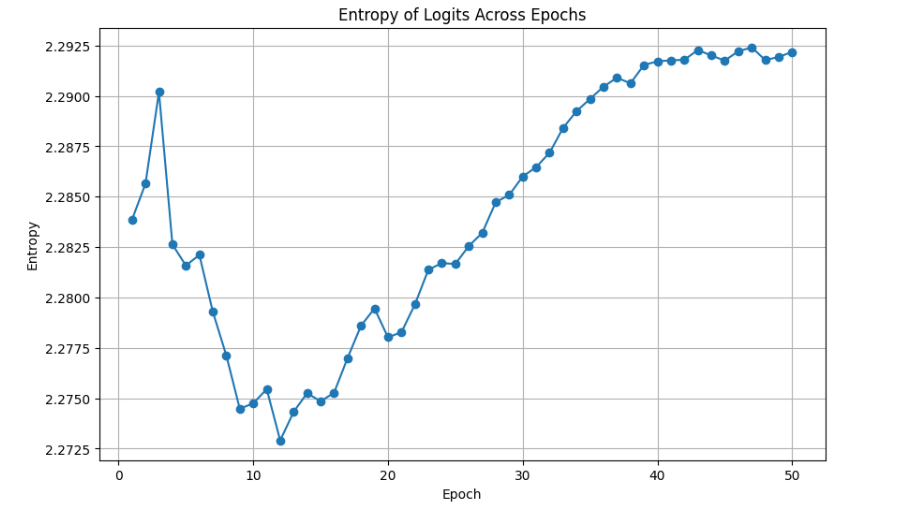
\includegraphics[width=0.7\textwidth]{images/entropy_m2.png}
    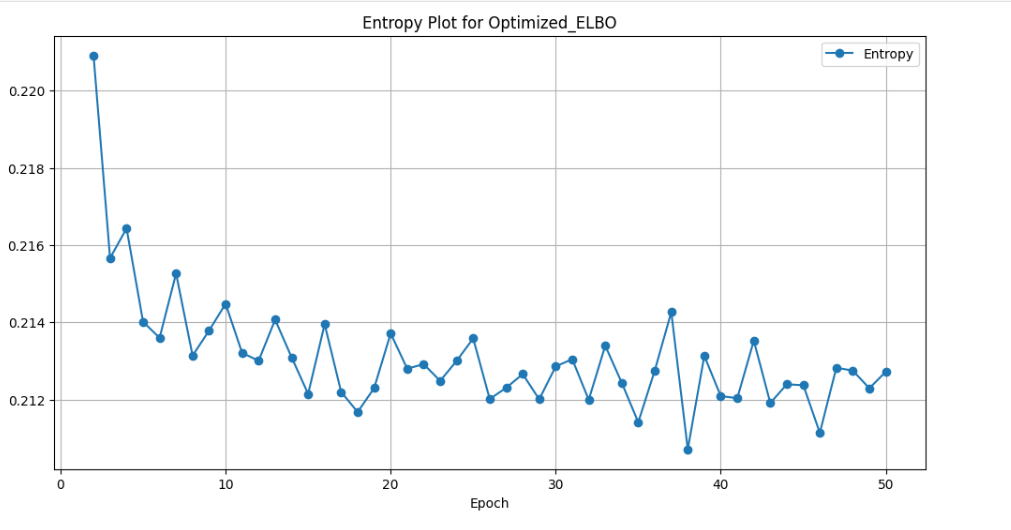
\includegraphics[width=0.7\textwidth]{images/Entropy_Optimized_elbo.png}
\end{itemize}

\subsection*{2. ELBO for Labeled Data Not Learning from Labels}
\begin{itemize}
    \item \textbf{Issue}: The original labeled ELBO in the M2 model fails to utilize label information effectively, as seen in Equation (6). Experimental results also show this leads to suboptimal classifier performance.
    \item \textbf{Experiment}:
    \begin{itemize}
        \item Compared the learning curves of the M2 model and the Optimized-Labeled ELBO (without cross-entropy loss in both cases) over 30 epochs.
        \item Results showed that the Optimized-Labeled ELBO consistently leveraged labeled data more effectively, enhancing classifier performance.
    \end{itemize}
    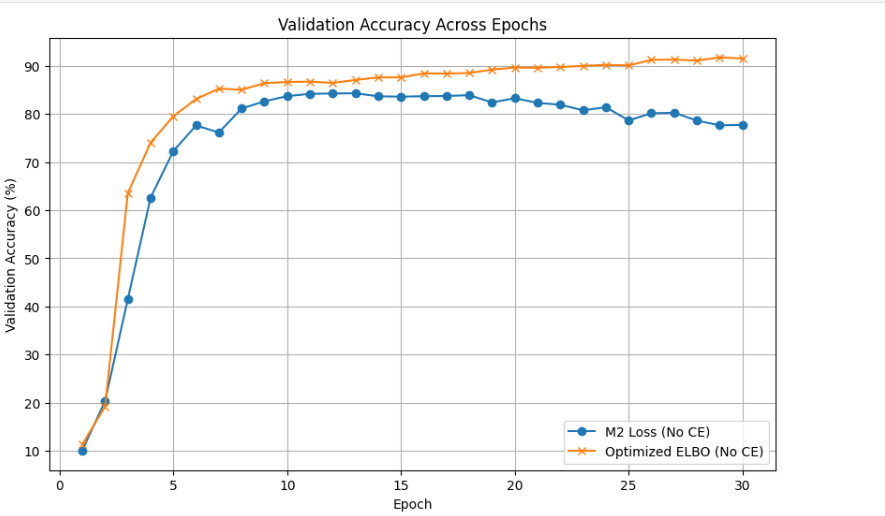
\includegraphics[width=0.7\textwidth]{images/val_acc_without_CE.png}
\end{itemize}

\section*{Conclusions}
\begin{enumerate}
    \item \textbf{Performance Improvements}:
    \begin{itemize}
        \item The Optimized-ELBO loss function demonstrated accuracy improvements on MNIST and modest gains on CIFAR-10.
        \item These improvements can be attributed to reduced classifier entropy, better decision boundary alignment, and enhanced utilization of labeled data.
    \end{itemize}
    \item \textbf{Entropy Reduction}: The proposed method successfully reduced the entropy of the classifier, leading to improved classification performance.
    \item \textbf{Labeled Data Utilization}: The Optimized-Labeled ELBO better utilized labeled data compared to the original M2 model.
    \item \textbf{Future Work}:
    \begin{itemize}
        \item For CIFAR-10, employing a deeper CNN architecture and advanced data augmentation could further enhance performance.
        \item Exploring additional regularization techniques and alternative priors may offer further insights into optimizing semi-supervised learning.
    \end{itemize}
\end{enumerate}

\section*{Bibliography}
\begin{enumerate}
    \item Olivier Chapelle, Bernhard Scholkopf, and Alexander Zien. Semi-supervised learning (Chapelle, O. et al., eds.; 2006) [book reviews]. \textit{IEEE Transactions on Neural Networks}, 20(3):542–542, 2009.
    \item Matthew D Hoffman and Matthew J Johnson. Elbo surgery: yet another way to carve up the variational evidence lower bound. In \textit{Workshop in Advances in Approximate Bayesian Inference, NIPS}, volume 1, page 2, 2016.
    \item Diederik P Kingma, Danilo J Rezende, Shakir Mohamed, and Max Welling. Semi-supervised learning with deep generative models. In \textit{Proceedings of the 27th International Conference on Neural Information Processing Systems-Volume 2}, pages 3581–3589, 2014.
    \item Ali Lotfi Rezaabad and Sriram Vishwanath. Learning representations by maximizing mutual information in variational autoencoders. In \textit{2020 IEEE International Symposium on Information Theory (ISIT)}, pages 2729–2734. IEEE, 2020.
    \item Yves Grandvalet and Yoshua Bengio. \textit{Semi-supervised learning by entropy minimization}. In \textit{CAP}, pages 281–296, 2005.
    \item Hanchen Xie et al. \textit{MUSCLE: Strengthening Semi-Supervised Learning via Concurrent Unsupervised Learning Using Mutual Information Maximization}. In \textit{2021 IEEE Winter Conference on Applications of Computer Vision (WACV)}, pages 2585–2594. IEEE, 2021.
    \item Müller et al. \textit{When Does Label Smoothing Help?}. In \textit{NeurIPS}, 2019.
\end{enumerate}


\section{Survey Section}

\subsection{Paper 1: Semi-Supervised Learning with Deep Generative Models}
\textbf{Authors:} Diederik P. Kingma, Danilo J. Rezende, Shakir Mohamed, and Max Welling  
\textbf{Published In:} Proceedings of the 27th International Conference on Neural Information Processing Systems, 2014  

\subsection*{Overview}
This foundational paper introduces semi-supervised learning frameworks using deep generative models, particularly the M1 and M2 architectures. The models combine variational autoencoders (VAEs) with discriminative classifiers, leveraging both labeled and unlabeled data. The approach provides a principled probabilistic framework for semi-supervised learning and demonstrates strong performance on various benchmarks.

\subsection*{Key Contributions}

\begin{enumerate}
    \item \textbf{M1 and M2 Architectures:}
    \begin{itemize}
        \item \textbf{M1:} A latent-variable generative model where \(z\) represents latent continuous features. A separate classifier is trained on these inferred latent variables.
        \item \textbf{M2:} A generative semi-supervised model combining the latent variable \(z\) and class labels \(y\), with joint training using the Evidence Lower Bound (ELBO).
    \end{itemize}
    
    \item \textbf{Objective:}  
    The semi-supervised objective integrates labeled and unlabeled data using the ELBO, enabling effective training of both the generative and inference models.

    \item \textbf{Key Insights:}
    \begin{itemize}
        \item Demonstrates how unlabeled data can improve classifier performance by leveraging generative modeling.
        \item Proposes scalable optimization techniques using stochastic gradient variational Bayes (SGVB).
    \end{itemize}
\end{enumerate}


\subsection{Paper 2: ELBO Surgery: Yet Another Way to Carve Up the Variational Evidence Lower Bound}
\textbf{Authors:} Matthew D. Hoffman and Matthew J. Johnson  
\textbf{Published In:} Workshop in Advances in Approximate Bayesian Inference, NIPS, 2016  

\subsection*{Overview}
This paper provides a detailed decomposition of the Evidence Lower Bound (ELBO), offering a systematic approach to analyze and address the shortcomings in variational inference (VI). It highlights specific issues with the ELBO in semi-supervised settings, particularly its inability to use labeled data effectively, and proposes modifications to enhance model performance.

\subsection*{Key Contributions}
\begin{enumerate}
    \item \textbf{ELBO Decomposition:}  
    The ELBO is decomposed into three terms for better understanding:
    \begin{itemize}
        \item \textbf{Reconstruction Term:} Measures how well the generative model reconstructs the data.
        \item \textbf{Prior Regularization:} Penalizes the divergence between the posterior and the prior.
        \item \textbf{Entropy Term:} Captures the level of uncertainty in the approximate posterior.
    \end{itemize}
    
    \item \textbf{The Good ELBO, Bad Inference Problem:}  
    The paper identifies that the classifier \( q_\phi(y|X) \) is not explicitly optimized using labeled data in the labeled ELBO, resulting in poor inference despite an optimized ELBO.

    \item \textbf{Proposed Adjustments:}  
    A new term is introduced to explicitly optimize \( q_\phi(y|X) \), ensuring that the labeled ELBO incorporates classification performance:
    \[
    \text{Modified ELBO}_{D_L}(X, y) = \text{ELBO}_{D_L}(X, y) - \alpha D_{\text{KL}}(\hat{p}(y|X) \| q_\phi(y|X)),
    \]
    where \(\alpha\) is a hyperparameter controlling the importance of classification loss.
\end{enumerate}

\subsection*{Strengths}
\begin{itemize}
    \item \textbf{Clear Diagnostic Framework:}  
    The decomposition of the ELBO provides a systematic way to identify and address its limitations.
    \item \textbf{Direct Optimizations:}  
    By explicitly incorporating classification loss, the proposed method effectively addresses the inference bottleneck.
\end{itemize}

\subsection*{Weaknesses}
\begin{itemize}
    \item \textbf{Limited Empirical Validation:}  
    The paper focuses on theoretical improvements and lacks extensive experimental results.
    \item \textbf{Not Generalizable:}  
    The proposed adjustment does not directly address entropy-related issues or mutual information in the unlabeled setting, making it less comprehensive for semi-supervised learning.
\end{itemize}
\subsection{Paper 3: Rethinking Semi–Supervised Learning in VAEs}  
\textbf{Authors:} Babak Esmaeili, Hao Wu, Sarthak Jain, Alican Bozkurt, Narayanaswamy Siddharth, Brooks Paige, Dana H. Brooks, Jennifer Dy, and Jan-Willem Meent  
\textbf{Published In:} The 22nd International Conference on Artificial Intelligence and Statistics (AISTATS), 2019  

\subsection*{Overview}  
This paper critically re-evaluates the assumptions underlying traditional approaches like the M2 model introduced by Kingma et al., after analyzing semi-supervised learning in Variational Autoencoders (VAEs). It introduces alternative formulations and explores methods to improve the generative and discriminative performance of semi-supervised VAEs.

\subsection*{Key Contributions}
\begin{enumerate}
    \item \textbf{Analysis of M2's Limitations:}
    \begin{itemize}
        \item Identifies key shortcomings in how labeled and unlabeled ELBOs are combined in the M2 framework.
        \item Highlights the misalignment between generative and discriminative objectives in traditional semi-supervised VAE approaches.
    \end{itemize}

    \item \textbf{Alternative Objectives:}
    \begin{itemize}
        \item Proposes new formulations to better integrate labeled and unlabeled data in a unified framework.
        \item Addresses critical issues, such as classifier entropy and mutual information between latent representations and labels.
    \end{itemize}

    \item \textbf{Insights into Regularization:}
    \begin{itemize}
        \item Discusses the role of regularization in semi-supervised learning.
        \item Provides theoretical insights into its impact on representation learning.
    \end{itemize}

    \item \textbf{Mathematical Framework:}
    \begin{itemize}
        \item The ELBO for labeled data is defined as:
        \[
        \text{ELBO}_{D_L}(X, y) = \mathbb{E}_{q_\phi(z|X, y)}[\log p_\theta(X|z, y)] 
        - D_{\text{KL}}(q_\phi(z|X, y) \| p(z)) + \log p_\theta(y). \tag{1}
        \]
        \item The ELBO for unlabeled data is:
        \[
        \text{ELBO}_{D_U}(X) = \mathbb{E}_{q_\phi(z, y|X)}[\log p_\theta(X|z, y)] 
        - D_{\text{KL}}(q_\phi(z|X) \| p(z)) - D_{\text{KL}}(q_\phi(y|X) \| p(y)). \tag{2}
        \]
        \item Highlights the mutual information term \( I_\phi(y; X) \):
        \[
        \mathbb{E}_{q(X)} \left[ D_{\text{KL}}(q_\phi(y|X) \| p(y)) \right] \geq I_\phi(y; X). \tag{3}
        \]
        \item Discusses entropy \( H(q_\phi(y|X)) \) as a factor influencing classification performance:
        \[
        H(q_\phi(y|X)) = -\mathbb{E}_{q_\phi(y|X)}[\log q_\phi(y|X)]. \tag{4}
        \]
    \end{itemize}

    \item \textbf{Unified Objective:}
    Proposes an updated objective function incorporating mutual information and entropy terms:
    \[
    J = \sum_{(X, y) \sim D_L} \text{ELBO}_{D_L}(X, y) + \sum_{X \sim D_U} \left[ \text{ELBO}_{D_U}(X) + \gamma I_\phi(y; X) - \beta H(q_\phi(y|X)) \right]. \tag{5}
    \]
    Here:
    \begin{itemize}
        \item \( \gamma \): Controls the weight of the mutual information term.
        \item \( \beta \): Controls the weight of the entropy term.
    \end{itemize}
\end{enumerate}




\end{document}
